%!TEX root = main.tex

\section{Objetivos}

Cada vez mais são utilizados sistemas \acrfull{iot} no meio industrial, como se pode verificar na figura \ref{fig:investment}, devido à sua flexibilidade de utilização e benefícios diretos que providenciam. 

\begin{figure}[ht]
	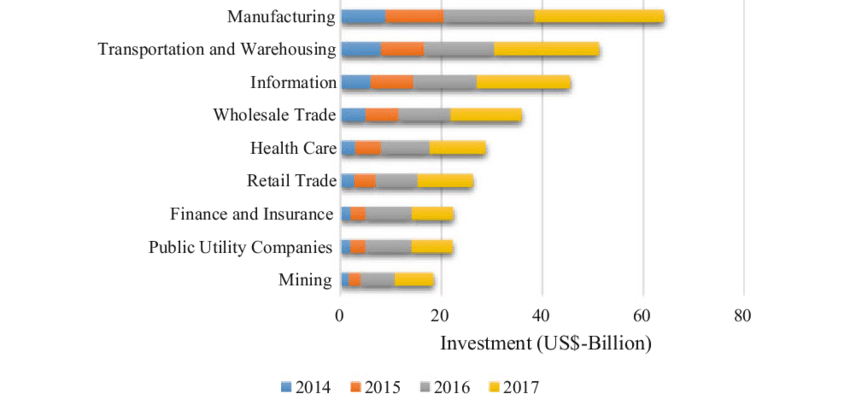
\includegraphics[width=\textwidth]{images/investments-in-IoT-solutions-by-industry.png}
	\caption{Investimento em \acrshort{iot} por indústria \parencite{cyberind4}}
	\label{fig:investment}
	\centering
\end{figure}

Para efeito deste projeto, definimos \acrshort{iot} como os dispositivos e serviços que conectam o meio industrial à Internet.

Os sistemas \acrshort{iot} trazem um conjunto de benefícios para as empresas e trabalhadores nas áreas industriais como, por exemplo \parencite{mendoza}:

\begin{itemize}
	\item Aumento de eficiência: a capacidade disponibilizada para automatizar permite otimizar as operações industriais
	\item Redução de erros: ao permitir a automatização de vários processos, os sistemas \acrshort{iot} permitem remover o erro humano, protegendo os trabalhadores e a empresa.
	\item \acrfull{pm}: os dispositivos \acrshort{iot} produzem uma panóplia de dados, que, quando devidamente analisados, permitem prever e evitar falhas, procedendo à manutenção de forma preditiva.
	\item Maior segurança: estes dados produzidos podem também ajudar a proteger os trabalhadores, mantendo o meio de trabalho dentro de parâmetros de segurança de forma constante, reduzindo a possibilidade de, entre outras situações, acidentes no trabalho.
	\item Redução de custos: tal como em outras áreas económicas, a aquisição de informação permite a uma redução de custos, através de maior eficiência, menos tempo de manutenção, melhor controlo de qualidade e menos erros no processo industrial, entre outros.
\end{itemize}

No entanto, estes sistemas produzem e acessam a dados cuja confidencialidade, integridade e disponibilidade devem ser garantidos, assim como a sua disponibilidade apenas para atores autenticados e autorizados. Por esta razão estes sistemas enfrentam frequentemente problemas de segurança que devem ser respondidos, resposta esta que varia dependendo do ataque executado, o que torna a implementação de mecanismos de segurança imperativa.

Desta forma pretendemos, com a implementação de um sistema pericial, detetar e identificar intrusões em sistemas IoT, permitindo a escolha da melhor abordagem para lidar com o ataque.





